\documentclass[fleqn,usenatbib]{mnras}
\usepackage{newtxtext,newtxmath}
\usepackage[T1]{fontenc}
\DeclareRobustCommand{\VAN}[3]{#2}
\let\VANthebibliography\thebibliography
\def\thebibliography{\DeclareRobustCommand{\VAN}[3]{##3}\VANthebibliography}

%%%%% AUTHORS - PLACE YOUR OWN PACKAGES HERE %%%%%
\usepackage{graphicx}	% Including figure files
\usepackage{amsmath}	% Advanced maths commands
\usepackage{xspace}
\usepackage{xcolor}
\usepackage{fontawesome}
\usepackage{listings}
\usepackage{changepage}
\usepackage{graphicx}
%%%%%%%%%%%%%%%%%%%%%%%%%%%%%%%%%%%%%%%%%%%%%%%%%%

%%%%% AUTHORS - PLACE YOUR OWN COMMANDS HERE %%%%%

% COMMENTS
\newcommand{\SB}[1]{{\textcolor{purple}{#1}}}

% NAMES
\newcommand{\Gaia}{\textit{Gaia}\xspace} % \Gaia

% STELLAR LABELS
\newcommand{\Teff}{$T_\mathrm{eff}$\xspace}
\newcommand{\logg}{$\log g$\xspace}
\newcommand{\feh}{$\mathrm{[Fe/H]}$\xspace}

% UNITS
\newcommand{\dex}{\,\mathrm{dex}}	% dex
\newcommand{\K}{\,\mathrm{K}}	% dex
\newcommand{\Msol}{\,\mathrm{M_\odot}} % Msol
\newcommand{\kpc}{\,\mathrm{kpc}}	% kpc
\newcommand{\Gyr}{\,\mathrm{Gyr}}	% Gyr
\newcommand{\Angstroem}{\,\text{\AA}}	% Angstroem
\newcommand{\kms}{\,\mathrm{km\,s^{-1}}}	% km/s

% GITHUB INFORMATION
\newcommand{\githubusername}{USERNAME}
\newcommand{\githubrepository}{REPOSITORY}
\newcommand{\codeicon}{{\faCloudDownload}}

%%%%%%%%%%%%%%%%%%%%%%%%%%%%%%%%%%%%%%%%%%%%%%%%%%

%%%%%%%%%%%%%%%%%%% TITLE PAGE %%%%%%%%%%%%%%%%%%%

% Title of the paper, and the short title which is used in the headers.
% Keep the title short and informative.
\title[Short title, max. 45 characters]{Stellar Ages for Galactic Archaeology with HERMES (GALAH)\thanks{All code, data, figures, and tables available at \url{https://github.com/\githubusername/\githubrepository}.}}

% The list of authors, and the short list which is used in the headers.
% If you need two or more lines of authors, add an extra line using \newauthor
\author[M. Bedford et al.]{
Marcus Bedford,$^{1}$\thanks{E-mail: u7312236@anu.edu.au}
and S. Buder$^{1,2}$
\\
% List of institutions
$^{1}$Research School of Astronomy and Astrophysics, Australian National University, Canberra, ACT 2611, Australia\\
$^{2}$ARC Centre of Excellence for All Sky Astrophysics in 3 Dimensions (ASTRO 3D), Australia
}

% These dates will be filled out by the publisher
\date{Accepted DD MM 2024. Received DD MM 2024; in original form 22 February 2024}

% Enter the current year, for the copyright statements etc.
\pubyear{2024}

% Don't change these lines
\begin{document}
\label{firstpage}
\pagerange{\pageref{firstpage}--\pageref{lastpage}}
\maketitle

% Abstract of the paper
\begin{abstract}
% CONTEXT
\textbf{Context:} Galactic Archaeology attempts to piece together the history and evolution of our Galaxy through information from today. With higher resolution spectroscopy from HERMES, accurate parallax from Gaia and asteroseismic data from K2, there is a wealth of new information from which to derive the mass and age of stars in the Milky Way. \newline
% AIMS
\textbf{Aims:} Comparing to the PARSEC isochrones, main sequence turn off (MSTO) stars will be fit using information provided from their spectra and further analysed in a Bayesian framework. Similarly, a model has been built to accurately predict the mass, and then consequently the ages of Red giants stars. These models will then be applied to unseen stars from the GALactic Archaeology with HERMES (GALAH) dr4.   \newline
% METHODS/ANALYSIS
\textbf{Methods/Analysis:} \newline
% RESULTS
\textbf{Results:} \newline
% CONCLUSIONS / IMPACT
\textbf{Conclusions / Expected Impact:} \newline
\href{https://github.com/\githubusername/\githubrepository}{\faGithub}
\end{abstract}

% Select between one and six entries from the list of approved keywords:
%https://academic.oup.com/DocumentLibrary/mnras/keywords.pdf
\begin{keywords}
techniques: spectroscopic -- stars: abundances -- keyword3 -- keyword4 -- keyword5 -- keyword6
\end{keywords}

%%%%%%%%%%%%%%%%%%%%%%%%%%%%%%%%%%%%%%%%%%%%%%%%%%

%%%%%%%%%%%%%%%%% BODY OF PAPER %%%%%%%%%%%%%%%%%%

\section{Introduction}

Obtaining accurate ages and masses for stars is an ongoing battle that improves through more precise data, increasingly accurate models and faster computers. The desire to have accurate and precise age and mass is fundamental to galactic Archaeology. Alongside other parameters such as chemical composition, position in the Milky Way, temperature and luminosity, age and mass will more concretely establish the evolution and composition of the Galaxy. Beyond this, understanding our spiral galaxy in great detail will allow further understanding of other similar galaxies. The difficulty of measuring a star’s age continues to hamper progress in Galactic studies (\citet{BlandHawthorn_Gerhard2016}). With giants being some of the most luminous objects in space the methodology 
described in this study for aging these and MSTO stars is highly applicable to more distant galaxies. 
\\
With high-precision data from GALAH dr4 we are in a good position to address the need for accurate and far reaching data. This study will explore two common methods for analysing stellar ages and masses: Isochrone fitting and Carbon and Nitrogen abundance. Both methods excel over a limited range of stars with isochrones being suited to the main sequence turn off and subgiants (\citet{Martigetal2016}) whilst extrapolating from Carbon and Nitrogen abundance is best for Red Giants. Combining both methods will allow this study to analyse more stars within the survey.

\subsection{Scientific Motivation and Context} \label{sec:intro_motivation}
Historically, The determination of accurate stellar ages and masses is notoriously difficult (\citet{linetal2018}). Unfortunately, time is not really a direct agent of change in stars, it is more a medium in which gradual changes occur (\citet{Soderblom2010}), making it difficult to determine age with precision. To date, the Sun is the only star with which we know age and mass to great accuracy. Beyond this, Asteroseismology is providing the next most accurate estimations of mass and age of red giants (\citet{Ness_2016}). The stars observed by K2 (\citet{2014Howell}) provide accurate asteroseismic information from a small portion of stars overlapped with GALAH spectroscopic data. This overlap provides a promising opportunity to train machine learning models on K2 stars that can then be applied to other stars in the survey.
\\
Previous papers have analysed various components of the Milky Way in great detail. One such paper by \citet{ciuca2021} looked closely at the chemical geography of the Galaxy stating a clear transition phase from the smaller chemically well-mixed thick to a larger thin disc with a metallicity gradient. This paper is also partly inspired by the work of \citet{2022Natur} who published fascinating work on the history of stellar evolution of the Galaxy by quantifying star age, stating
\\
\begin{adjustwidth}{1cm}{}
    \textit {"Star formation rate of the old disks reached a prominent maximum at \(\sim\)11.2Gyr ago, apparently just when the merger with the Gaia Enceladus was complete, and then continuously declined with time."\newline}
\end{adjustwidth} 

For the most part, age estimates from spectroscopic surveys have been determined for stars before or just after MSTO and subgiants. In that regime, stellar evolutionary isochrones are well separated (\citet{Ness_2016}). Furthermore, subgiants have been described as the best practical tracers of Galactic archaeology as their elemental compositions determined from spectra, accurately reflect their birth material composition billions of years ago (\citet{2022Natur}). Isochrones have provided a foundation for astronomers to compare theoretical and observational data over many years, notably for this study \citet{linetal2018}, \citet{2022Natur}, \citet{ciuca2021}, \citet{Jorgensen2005}. Whilst Isochrone fitting is historically a hugely popular method for stellar analysis, quantifying their statistical reliability in view of the observational uncertainties, is relatively newer and within the domain of Bayesian analysis (\citet{Jorgensen2005}). 

On the other hand, masses of red giant stars can be well predicted from their photospheric carbon and nitrogen abundances in conjunction with information on log g, \(T_{eff}\) and [Fe/H] (\citet{Martigetal2016}). Furthermore, ages of giants can be directly inferred from their masses. Giants make excellent subjects for a galactic survey as their higher luminosity allows them to be seen from great distances. Because the [C/N] ratio in the core and the depth reached by the first dredge-up depend on stellar mass, the final [C/N] ratio at the surface depends on stellar mass (\citet{Martigetal2016}). a model will be trained and tested on stars with ages derived accurately from K2 Asteroseismic data and then applied to the remaining stars within the cut from GALAH.

\subsection{Objective of This Research} \label{sec:intro_objectives}
This study will apply, and where possible improve upon, previous stellar aging methods to the set of stars within the cut of GALAH dr4. This study will pay particular interest to stars on the extreme edges of the Z axis of the Galactic plane where less information is currently available, to help provide a more encompassing map of Galactic geography. A recent study by \citet{2022Natur} using isochrone fitting on a broad area of the Milky Way set the benchmark for this study claiming, "Such high precision has never been reached for any large sample of stars before", achieving an age uncertainty of only 7.5\%. However, 90\% of the stars considered in the survey were within \(-1.2kpc < Z < 2kpc\)  of the Z axis of the galactic plane. The width of stars observed by GALAH reaches far beyond this.  \\
The updated PAdova tRieste Stellar Evolutionary Code (PARSEC) v2.0 (\cite{Costaetal2019a, Costaetal2019b,Nguyenetal2022}) will be used in a Bayesian framework with priors relating to initial mass and ... to find the most likely age and mass with uncertainty. Whilst there are many Isochrones that as the Yonsei-Yale models (\citet{Yi2003}) that would do a similar job, PARSEC is best suited to lower and intermediate mass stars. PARSEC v2.0 provides isochrones ranging 6 initial metallicities from \(0.004 \leq \mathrm{[X/H]} \leq 0.017\), initial mass ranging from \(0.09\leq \Msol\leq14\) as well the inclusion of 7 initial rotation values ranging from \(0\leq \Omega/\Omega_{crit}\leq 0.99\). 
\begin{itemize}
    \item To which extend is ...?
    \item How can we best ...?
    \item What physical process drive ...?
    \item How strong is the correlation between ... and can we explain this with a physical causality?
\end{itemize}

\subsection{Structure of This Paper} \label{sec:intro_structure}

Similar to a table of contents, tell the reader where to find what:

We present the data used for this study in Sec.~\ref{sec:data}, together with a description of different quality cuts that we perform. We then describe our analysis approach in Sec.~\ref{sec:analysis}. We present our results in Sec.~\ref{sec:results} and put them into context during our discussion in Sec.~\ref{sec:discussion}. We conclude our stud and give an outlook in Sec.~\ref{sec:conclusions}.

\section{Data} \label{sec:data}
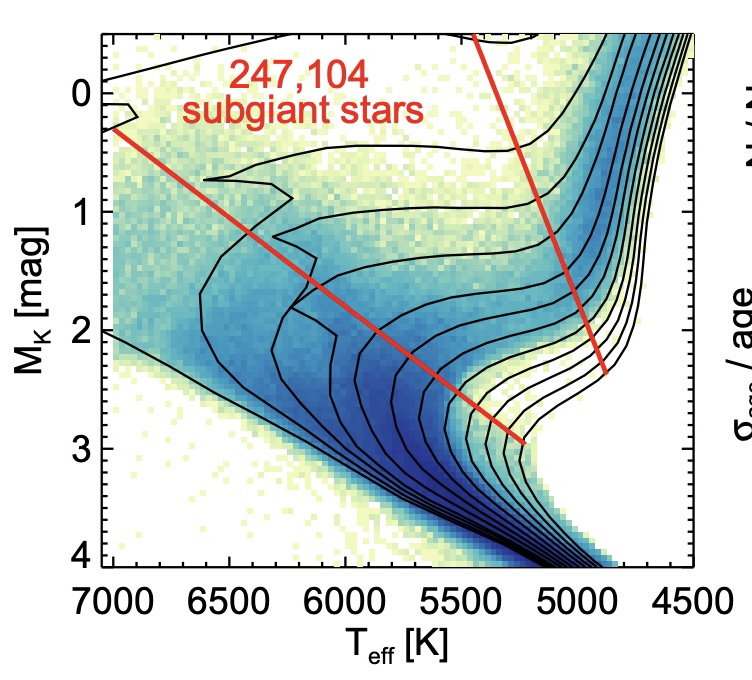
\includegraphics[scale=0.3]{Image 11-3-2024 at 1.09 pm 2}
This section should describe all the data that you used. Try to explain everything that is necessary for a reader to understand how the data was obtained, but do not go overboard with the details:  (it is not important that button X was pressed)

Normally the next section describes the techniques the authors used.
It is frequently split into subsections, such as Section~\ref{sec:maths} below.

Whenever you perform any cuts or selection of the data, you need to include this in the manuscript. An easy way could be to use an equation, like Eq.~\ref{eq:basic_cuts}:
\begin{equation} \label{eq:basic_cuts}
\text{Basic cuts} = 
\begin{cases}
\texttt{flag\_sp} = 0, \texttt{flag\_fe\_h} = 0, \\
\texttt{flag\_X\_fe} = 0 \text{ for each used element X} \\
\end{cases}
\end{equation}
 For example that we define the absolute \textit{chemical abundance} A(X) as the logarithmic ratio of the number densities $N$ of elements X to hydrogen, that is 
\begin{equation}
\mathrm{A(X)} = \log_{10} \frac{N_\text{X}}{N_\text{H}} + 12.   
\end{equation}

Comparing this ratio with the Solar ($\odot$) one would lead us to 
\begin{equation}
\mathrm{[X/H]} = \mathrm{A(X)} - \mathrm{A(X)}_\odot    
\end{equation}
and comparing that to iro\footnote{Iron is used because it is one of the elements with the most lines in neutral and ionised states in stellar spectra and a lot of element number densities scale with it.} as an often-used metallicity tracer would lead us to
\begin{equation}
\mathrm{[X/Fe]} = \mathrm{[X/H]} - \mathrm{[Fe/H]}.
\end{equation}


\section{Analysis} \label{sec:analysis}

\section{Results} \label{sec:results}

\section{Discussion} \label{sec:discussion}

How you structure this section is again totally up to you. I personally like to remind myself of the objectives of the research from Sec.~\ref{sec:intro_objectives}.

The aim of our study is to find ... (see Sec.~\ref{sec:intro_objectives})

\subsection{Objective 1 (replace that with a meaningful title)} \label{sec:discussion_objective_1}

\subsection{Objective 2 (replace that with a meaningful title)} \label{sec:discussion_objective_2}

\subsection{Objective 3 (replace that with a meaningful title)} \label{sec:discussion_objective_3}


\section{Conclusions} \label{sec:conclusions}

In my opinion, this is a personal choice, but roughly half of the researchers use a final section to briefly summarise what has been done, and describe the final conclusions which the authors draw from their work.

%%%%%%%%%%%%%%%%%%%%%%%%%%%%%%%%%%%%%%%%%%%%%%%%%%
\newpage

\section*{Acknowledgements}

Here you can thank helpful colleagues, acknowledge funding agencies, telescopes and facilities used etc. I personally also include a statement that pays respect to the traditional custodians of the Country that this work was done from. I for example, start my acknowledgements like this:

We acknowledge the traditional owners of the land on which the AAT and ANU stand, the Gamilaraay, the Ngunnawal and Ngambri people. We pay our respects to elders past and present and are proud to continue their tradition of surveying the night sky in the Southern hemisphere.

%%%%%%%%%%%%%%%%%%%%%%%%%%%%%%%%%%%%%%%%%%%%%%%%%%

\section*{Facilities}

\textbf{\Gaia: } This work has made use of data from the European Space Agency (ESA) mission \Gaia (\url{http://www.cosmos.esa.int/gaia}), processed by the \Gaia Data Processing and Analysis Consortium (DPAC, \url{http://www.cosmos.esa.int/web/gaia/dpac/consortium}). Funding for the DPAC has been provided by national institutions, in particular the institutions participating in the \Gaia Multilateral Agreement. 
\textbf{Other facilities:} This publication makes use of data products from the Two Micron All Sky Survey \citep{Skrutskie2006} and the CDS VizieR catalogue access and Aladin visualisation tool \citep{Vizier2000,Aladin2000}.

%%%%%%%%%%%%%%%%%%%%%%%%%%%%%%%%%%%%%%%%%%%%%%%%%%

\section*{Software}

The research for this publication was coded in \textsc{python} (version 3.7.4) and included its packages
\textsc{astropy} \citep[v. 3.2.2;][]{Robitaille2013,PriceWhelan2018},
\textsc{IPython} \citep[v. 7.8.0;][]{ipython},
\textsc{matplotlib} \citep[v. 3.1.3;][]{matplotlib},
\textsc{NumPy} \citep[v. 1.17.2;][]{numpy}, and
\textsc{scipy} \citep[version 1.3.1;][]{scipy}.
We further made use of \textsc{topcat} \citep[version 4.7;][]{Taylor2005};

%%%%%%%%%%%%%%%%%%%% REFERENCES %%%%%%%%%%%%%%%%%%
\bibliographystyle{mnras}
\bibliography{bibliography} % if your bibtex file is called example.bib
%%%%%%%%%%%%%%%%%%%%%%%%%%%%%%%%%%%%%%%%%%%%%%%%%%

\newpage
%%%%%%%%%%%%%%%%% APPENDICES %%%%%%%%%%%%%%%%%%%%%

\appendix

\section{Before you get started -- Delete this section before submission!}

\subsection{Expectations}

\subsubsection{Marking Guidelines}

Because this research will be marked, I strongly recommend you to familiarise yourself with the guidelines that you will get for the specific research.

The markers (which will likely include at least one person outside of my research area) are following the \textit{Marking Guidelines} and will be looking for ways to \textit{tick off} the specific criteria for each of the marks. Some of these marks will be given based on my assessment of independence, persistence, showing initiative etc.

\subsubsection{Running Notes and Deadlines}

Writing down plans, action items, and thoughts in general is extremely important. You can of course do that with pen and paper if you prefer. Otherwise, you can also create a \href{https://docs.google.com}{GoogleDoc} to document this or use the end of this document (Sec.~\ref{sec:running_notes}). In any case, please add the deadlines in Table~\ref{tab:deadlines}.

\begin{table}
	\centering
	\caption{When is what due?}
	\label{tab:deadlines}
	\begin{tabular}{lll} % four columns, alignment for each
		\hline
		Deadline & Week & Actual Date \\
		\hline
		Literature Review     & 6 & DD MM YY\\
		Final Presentation    & 11 & DD MM YY\\
		Final Report          & 12 & DD MM YY\\
		\hline
	\end{tabular}
\end{table}

\subsubsection{Communication and meetings}

\begin{itemize}
    \item I will make time to meet every student for \textit{at least} one hour per week. I prefer a scheduled meeting, but am happy to have impromptu meetings as well.
    \item Similar to the big tech companies, I will give you bonus marks if you try different approaches or make mistakes and tell me what you learned from them. If you are getting stuck with your research (for example coding), try to find a solution yourself (within a reasonable time, e.g. a code issue should be fixed within less than 30 minutes). Also consider asking your fellow students, feel free and strongly encouraged to ask me. The research project is too short to wait a whole week to wait until our next meeting to ask a question. 
    \item I ask my students to join the weekly group meetings (currently Thursdays 3-4pm in AITC1). This will be a great way to learn more about science and how it is done. In the current format, the group meeting rotates between (1) everyone-brings-a-plot, (2) paper-discussion, (3) skillsharing, and (4) expert talk sessions.
\end{itemize}

\subsubsection{Coding}

I am not a great coder myself - so I will not look down on any code that you write. But just like myself, I encourage you to always strive to improve yourself. There are a few ways to do that:
\begin{itemize}
    \item GitHub Copilot or ChatGPT are great ways to improve your coding (and commenting code). You can always ask these tools to improve your code and properly comment it (in most cases these tools will actually be able to help - but you have to check if the code still does what it is supposed to do).
    \item Automate your code: Use classes and functions with arguments. Whenever you copy code to apply it twice, this should be in a function (again the above programs can help you if you are new to coding).
    \item Use \textsc{pandas.DataFrame} or \textsc{astropy.table.Table} when working with large data collections. They have a lot of functionalities, like joining tables or visualising data easily.
    \item Save your results. This avoids to rerun expensive computations. Try to save your results in a useful format, for example FITS files.
    \item Make sure that you can repeat your measurements. When you share your code it should produce the same output independent of who is using it. When running code with random input (e.g. numpy.random), you can use the numpy.seed function.
\end{itemize}

\subsubsection{Figures}

Visualising your results is one of the most important parts of scientific communication and presentation. A lot of people will decide to read your paper (or not) based on a quick read of the abstract and looking at your figures (I am guilty of that myself). Great figures will also be picked up more often by other researchers in their own scientific communication (nobody will show an overly complicated and busy plot with too small font and a bad color choice).

\begin{itemize}
    \item Every figure needs axis labels
    \item The font size of everything on the figure should be at least as large as that of the normal text of the manuscript
    \item Plots with multiple panels need panel labels a), b) etc. and should share the same axis limits (where possible), see Sec.~\ref{sec:figures}
    \item scatter vs. 2D-histogram vs. contour:
    \begin{itemize}
        \item If you only show a few points, plt.scatter is the way to go
        \item For more than 50+ points, you should switch to a histogram plot (plt.hist2d)
        \item If you want to show multiple samples, try to use either contour plots or a combination of plt.hist2d in the background
    \end{itemize}    
    \item You can either use \textsc{figures} with columnwidth for a small figures or large \textsc{figures*} with textwidth.
\end{itemize}

\subsection{Finding and Writing Your Research Story}

Scientific writing can be incredibly difficult. There are different ways to guide your thinking that you could try in case you feel stuck:
\begin{itemize}
    \item Prepare a presentation with 10 slides that include the motivation, data, analysis, results, discussion, and a summary. I have always found this incredibly useful to find my \textit{story} and identify the key results and their impact.
\end{itemize}

\subsection{Useful Software}

\subsubsection{Finding and Managing References}

\begin{itemize}
    \item \href{https://ui.adsabs.harvard.edu}{ADS} is a website that allows you to search for papers with keywords. It also includes the necessary information to create a bibliography entry and find the actual paper PDF (and even its source code) on the journal website or the arXiv.
    \item \href{https://arxiv.org}{arXiv} is a website where researchers upload their papers with free access to allow others to see their science.
    \item \href{https://bibdesk.sourceforge.io}{BibDesk} is a program that allows you to save and search your references in a useful list. You can also store the location of the PDFs for each paper, so that you do not have to search for it on your computer (filenames can be quite random). You can import or store multiple bibliographies, for example as *.bib file, and upload them into overleaf.
\end{itemize}

\subsubsection{GitHub}

As a proponent of open, repeatable, and inclusive science, I encourage you to link to your GitHub repository, where the public can access your code and results. For this, you have to update the commands for \githubusername\xspace and \githubrepository\xspace in the preamble.

\subsubsection{Astronomical software / websites}

\begin{itemize}
    \item The CDS VizieR catalogue access tool \citep{Vizier2000} 
\end{itemize}


\subsubsection{TOPCAT}

\href{https://www.star.bris.ac.uk/~mbt/topcat/}{\textsc{TOPCAT}} by 



\section{Making great figures} \label{sec:figures}

\begin{lstlisting}[language=Python, caption=How to create a figure with 2 panels]
# define keywords like a fontsize
mfs = 15

f, gs = plt.subplots(1,2,sharex=True)
# sharex adjust the xlim to be the same

# Panel a)
ax = gs[0]
s = ax.plot(xdata, ydata, c = colordata)
ax.set_xlabel(X Label / Unit, fontsize=mfs)
ax.set_ylabel(Y Label / Unit, fontsize=mfs)
cbar = plt.colorbar(s,ax=ax)
cbar.set_label(Label / Unit, fontsize=mfs)

# Panel b)
ax = gs[1]
s = ax.plot(xdata, ydata, c = colordata)
ax.set_xlabel(X Label / Unit, fontsize=mfs)
ax.set_ylabel(Y Label / Unit, fontsize=mfs)
cbar = plt.colorbar(s,ax=ax)
cbar.set_label(Label / Unit, fontsize=mfs)

# Limit the white space
plt.tight_layout()

# Save the figure in a reasonable quality
# For *.png: bbox_inches='tight',dpi=300
# For *.pdf: avoid for scatter plots
plt.savefig(figures/useful_name.pdf)
\end{lstlisting}


\section{Useful LaTeX information} \label{sec:latex_information}

Below I am including a few examples of how to use maths, figures, and tables in \LaTeX. For a full user guide, please see the \texttt{mnras\_guide.tex}.

\subsection{Maths, Equations, and Units}
\label{sec:maths} % used for referring to this section from elsewhere

Simple mathematics can be inserted into the flow of the text, for example $v=220\,\mathrm{km\,s^{-1}}$. If you will use a unit a lot, it can come in handy to define it as a command, for example \textbackslash Teff, in the preamble, so that you can use it as \Teff, \logg, and \feh.

More complicated expressions should be entered as a numbered equation:

\begin{equation}
    x=\frac{-b\pm\sqrt{b^2-4ac}}{2a}.
	\label{eq:quadratic}
\end{equation}

Refer back to them as e.g. equation~(\ref{eq:quadratic}).

\subsection{Figures and tables}

Figures and tables should be placed at logical positions in the text. Figures are referred to as e.g. Fig.~\ref{fig:example_figure_small} or Figs.~\ref{fig:example_figure_small}-\ref{fig:example_figure_large}, and tables as e.g. Table~\ref{tab:example_table}.

% Example figure
\begin{figure}
	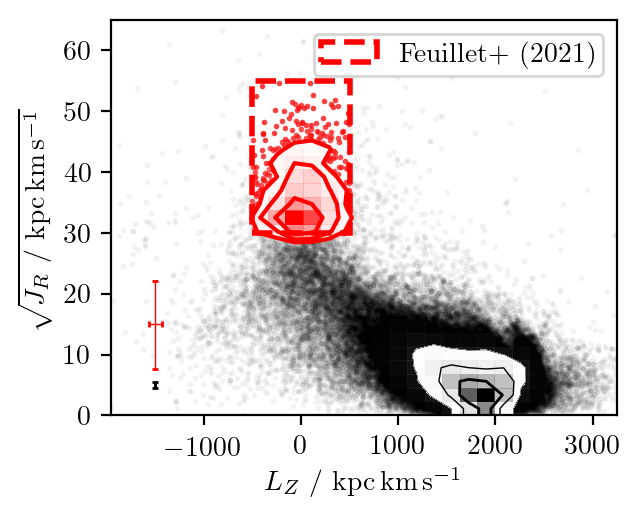
\includegraphics[width=\columnwidth]{figures/placeholder_columnwidth.png}
    \caption{This is a small example figure. Captions appear below each figure.
	Give enough detail for the reader to understand what they're looking at,
	but leave detailed discussion to the main body of the text.}
    \label{fig:example_figure_small}
\end{figure}

% Example figure
\begin{figure*}
	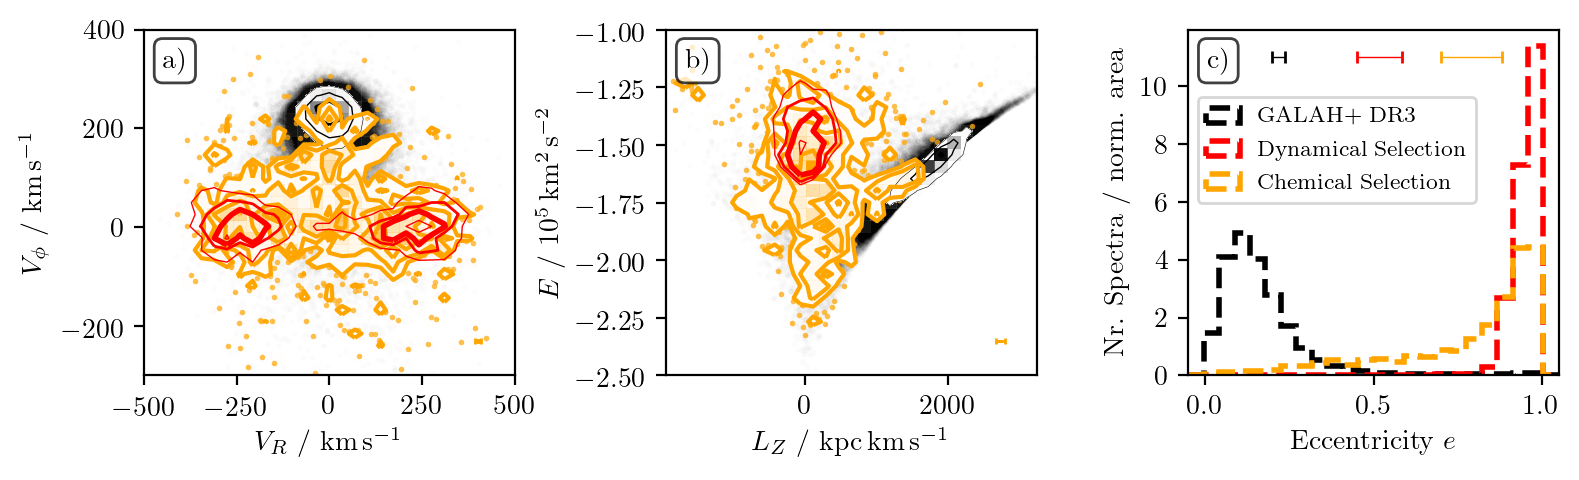
\includegraphics[width=\textwidth]{figures/placeholder_textwidth.png}
    \caption{This is a large example figure. Captions appear below each figure.
	Give enough detail for the reader to understand what they're looking at,
	but leave detailed discussion to the main body of the text.}
    \label{fig:example_figure_large}
\end{figure*}

% Example table
\begin{table}
	\centering
	\caption{This is an example table. Captions appear above each table.
	Remember to define the quantities, symbols and units used.}
	\label{tab:example_table}
	\begin{tabular}{lccr} % four columns, alignment for each
		\hline
		A & B & C & D\\
		\hline
		1 & 2 & 3 & 4\\
		2 & 4 & 6 & 8\\
		3 & 5 & 7 & 9\\
		\hline
	\end{tabular}
\end{table}

\section{Running Notes} \label{sec:running_notes}

%%%%%%%%%%%%%%%%%%%%%%%%%%%%%%%%%%%%%%%%%%%%%%%%%%
\label{lastpage}
\end{document}